\section{Consensus}

Nodes proposes value and they must agree on one of these values.

\paragraph{Key problem} Solve total order broadcast, atomic commit, reliable broadcast

\subsection{Properties}

\begin{description}
	\item[Validity] Any value decided is a value proposed
	\item[Agreement] No two correct nodes decide differently
	(in a \textbf{uniform consensus}, node does not need to be correct)
	\item[Termination] Every correct node eventually decides
	\item[Integrity] A node decides at most once
\end{description}

\begin{lstlisting}[caption={Consensus interface}]
Request: <cPropose | v>
Indication: <cDecide | v>
\end{lstlisting}


\subsection{Hierachical Consensus}

\begin{itemize}
    \item Use perfect failure detector $P$ and a best-effort broadcast $BEB$
    \item Each node stores its \texttt{proposal} and the identifier of the last
    adopted proposer in \texttt{lastprop}.
    \item Loop through rounds $1$ to $N$
        \begin{tabular}{m{1.3cm}m{13cm}}
            Round $i$ &
        \begin{itemize}
            \item node $i$ is leader and broadcasts and decides its proposal $v$
            \item Other nodes adopt $i$ proposal $v$ (save it in lastprop) or
                detect crash of $i$.
            \item[$\to$] Future rounds will only propose $v$
        \end{itemize}
    \end{tabular}
\end{itemize}

\subsubsection{Orphan message issue}

Problem is that broadcast can be delayed and the leader crash
and a node can receive two proposal in the next round. It will
therefore affect future round.

\begin{figure}[!ht]
    \centering
    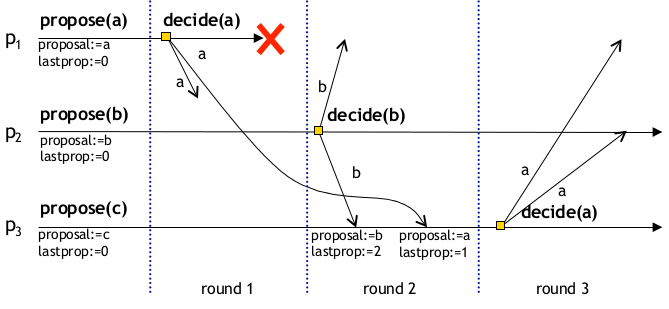
\includegraphics[width=8cm]{img/orphan.png}
    \caption{Orphan}
\end{figure}
\FloatBarrier{}

\paragraph{Solution}

Counter measure $\to$ ranking of the node based on there identifier
($p_1>p_2>p_3>\ldots$)

$\Rightarrow$ Adopt if proposer $p$ is ranked lower than lastprop otherwise $p$ has
crashed and should be ignored

\subsubsection{Implementation}

    \begin{lstlisting}[caption={Hierachical consensus}, mathescape]
upong event <Init> do
    detected :=  $\emptyset$
    round     := 1
    proposal := $\perp$ // last adopted proposal
    lastprop := 0  // last adopted proposer id
    for i=1 to N do
        broadcast[i] := delivered[i] := false

upon event <crash | $p_i$ do
    detected := detected $\cup$ {rank($p_i$)}

upon event <cPropose | v> do
    if proposal = $\perp$ then // set node's initial proposal unless it already has
        proposal := v

upon round = rank(self) and    // if I am leader
     broadcast[round] = false and   // trigger once per round
     proposal != $\top$ do    // trigger if I have proposal

    broadcast[round] := true
    trigger <cDecide | proposal>    // permanently decide
    trigger <bebBroadcast | (DECIDED, round, proposal)>

upon event <bebDeliver | $p_i$, (DECIDED, r, v)> do
    if r > lastprop then // invariant: only adopt newer than what you have
        proposal := v
        lastprop := r
    delivered[r] := true

upon delivered[round] or round $\in$ detected do
    round := round + 1  // next round if deliver or crash
\end{lstlisting}


\subsubsection{Correctness}
\begin{itemize}
	\item Validity? $\to$ Always decide own proposal or adopted value
	\item Integrity? $\to$ Rounds increase monotonically, node only
	decide when leader.
	\item Termination? $\to$ Every correct node makes it to the round it
	is leader in:
	\begin{itemize}
		\item If some leader fails, completeness of $P$ ensure progress.
		\item If leader correct, validity of BEB ensures delivery.
	\end{itemize}
	\item Agreement? $\to$ take correct leader with minimum id $i$.
        \begin{itemize}
            \item By termination it will decide $v$ and $v$ will be BEB
            \item[$\to$] Every correct node adopts $v$ no older proposal
                can override the adoption
        \end{itemize}
\end{itemize}

\textbf{Failure-torerant up to N-1}

\subsubsection{Formalism}
\begin{lstlisting}[caption={Hierarchical consensus}, mathescape]
$x_i$ := proposal
for r:=1 to N do
    if r=i then
        forall j in 1..N do
            send <val, $x_i$, r> to $P_j$;
        decide $x_i$
    if collect <val, x', r> from r then
        $x_i$ := x';
end
\end{lstlisting}

\subsection{Uniform consensus}
To reach uniform consensus, we move the decision to the end.

\begin{lstlisting}[caption={Uniform Hierarchical consensus with P}, mathescape]
$x_i$ := input
for r:=1 to N do
    if r=i then
        forall j in 1..N do
            send <val, $x_i$ , r> to $P_j$;
    if collect <val, x', r> from r then
        $x_i$ := x';
end
decide $x_i$
\end{lstlisting}

\subsubsection{With inaccurate FD}

\begin{figure}[!ht]
    \centering
    \begin{tabular}{m{8cm}m{8cm}}
        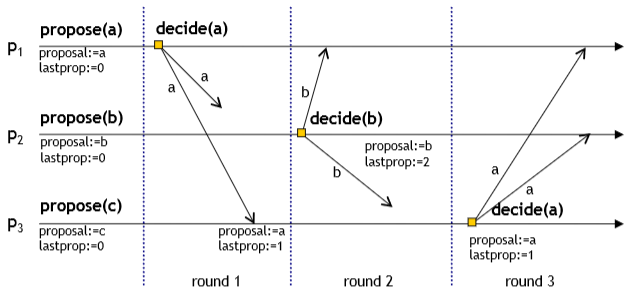
\includegraphics[width=8cm]{img/hc_fd.png} &
        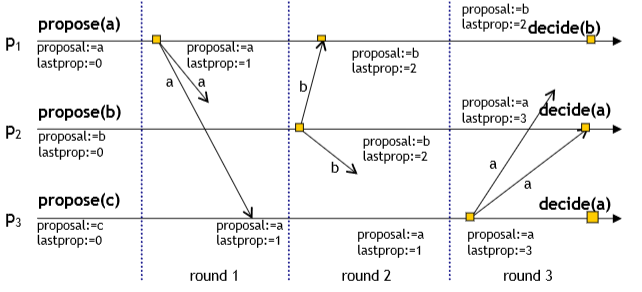
\includegraphics[width=8cm]{img/uhc_fd.png} \\
        p2 suspect p1, p3 suspect p2 (nonuniform consensus) &
        p2 suspect p1, p3 suspect p2, p1 suspect p3 (uniform consensus)\\
        \multicolumn{2}{c}{$\Rightarrow$ Doesn't work with innacurrate FD}
    \end{tabular}
        \caption{Inaccuracy with failure detector}
\end{figure}
\FloatBarrier{}

\textbf{The algorithm doesn't work with inaccurate FD}

\subsubsection{With Strong failure detector}

The algorithm works with a $S$ (strong detector). The difference between
Strong detector (weaker than $P$) and a Perfect detector comes from the
accuracy w.r.t one node.

\paragraph{Correctness}
\begin{itemize}
	\item Validity? $\to$ Always decide own proposal or adopted value
	\item Integrity? $\to$ Rounds increase monotonically, node only
	decides once in the end.
	\item Termination? $\to$ Every correct node makes it to the last round
	\begin{itemize}
		\item If some leader fails, completeness of $S$ ensures progress.
		\item If leader correct, validity of BEB ensures delivery.
	\end{itemize}
	\item Uniform agreement? $\to$ take an accurate correct leader with id $i$.
        \begin{itemize}
            \item By weak accuracy (S) and termination such a node exists
                and it will BEB $v$
        \end{itemize}
\end{itemize}


\subsubsection{With Eventual failure detector}
Eventually perfect detector cannot solve consensus with resilience $t \geq n/2$

%Proof?
\begin{itemize}
	\item Rotating coordinator from before will not work because
	\enquote{eventually} might be after the first $N$ rounds
	\item The idea is to rotate forever and eventually all nodes
	correct w.r.t. 1 coordinator (coordinator's value becomes
	agreed value)
\end{itemize}

\paragraph{Termination}
There will be a bound on the number of failures $\to$ less ($f<n/3$) than a third
can fail. This will allow to decide using majority.

\begin{enumerate}
	\item Everyone send vote to coordinator $C$
	\item $C$ picks majority vote $V$, and broadcasts $V$
	\item Every node get broadcast, change vote to $V$
	\item Change coordinator $C$ and go to 1
\end{enumerate}

\begin{lstlisting}[caption={Rotate coordinator for $\Diamond S$}, mathescape]
$x_i$ := input
r=0
while true do
begin
    r := r + 1
    c := (r mod n) + 1  // rotate to coordinator c
    send <value, $x_i$, r> to $p_c$ // all send value to coord

    if i==c then  // coord only
    begin
        msgs[0]:=0; msgs[1]:=0;    // reset 0 and 1 counter
        for x:=1 to N-f do
        begin
            receive <value, V, R> from q  // receive N-f msgs
            msgs[V]++;       // increase relevant counter
        end
        if msgs[0] > msgs[1] then v := 0 else v := 1 end // choose majority value
        if msgs[0]==0 or msgs[1]==0 then d := 1 else d := 0 end // all N-f same ?
        forall j do send <outcome, v, r> to $p_j$ // send v to all
    end

    if collect<outcome, v, r> from $p_c$ then   // collect value from coord
    begin
        $x_i$ := v  // adopt v
        if d and i!=0 then begin decide(v); i:=0; end
    end
end
\end{lstlisting}

\begin{itemize}
    \item If at least $n-f$ nodes vote $V$ in round $r$, every leader will see
    a majority for $V$ in all rounds > r.

        \paragraph{Proof}:
        \begin{itemize}
            \item We know that at most $f$ nodes don't vote $V$
            \item We also know $n/3<(n-f)/2$ (because $f<n/3$ implies $n-f>2n/3$)
                $\to f<(n-f)/2$ (because $f<n/3$ and $n/3<(n-f)/2$)
            \item So less than half of any $n-f$ nodes do not vote $V$
        \end{itemize}
\end{itemize}


\section{Terminating Reliable Broadcast (TRB)}

With normal reliable broadcast, no idea when or if a message will be delivered.

$\Rightarrow$ In TRB, sender broadcast $M$ and receiver await delivery $M$. All
nodes either deliver $M$ or \enquote{abort} (special sender faulty message <SF>)

TRB requires synchrony!

\begin{lstlisting}
Request: <trbBroadcast | src, m>
Request: <trbBroadcast | src, m>
\end{lstlisting}

\subsection{Property}
\begin{description}
	\item[TRB1. Termination] Every correct node eventually delivers one message
	\item[TRB2. Validity] If correct src sends $m$, then src will deliver $m$
	\item[TRB3. Uniform agreement] If any node delivers $m$, then every correct node
	eventually delivers $m$
	\item[TRB4. Integrity] If a node delivers $m$, then either $m=<SF>$ or $m$ was
	broadcast by src.
\end{description}

\subsection{Consensus based TRB}
Src RB broadcast $m$ (deliver <SF> if src is suspected by $P$)
\begin{itemize}
	\item Src BEB broadcast $m$
	\item Nodes propose whichever comes first: crash suspicion(<SF>) or
	BeB delivery from src (M)
	\item Deliver consensus decision
\end{itemize}


\subsubsection{Hardness}
\begin{itemize}
    \item $consensus \preceq TRB$ $\Rightarrow$ can't implement TRB in asynchronous networks.
    \item $ P \preceq TRB \land TRB \preceq P \Rightarrow TRB \simeq P$: can't
    implement TRB in eventually synchronous systems (with $\Diamond P$)
\end{itemize}

\subsubsection{Correctness}
TODO

\section{Total order broadcast (consensus)}

The order imposed by causal broadcast is partial. Some message might
be delivered in different order by different process.

With \textbf{total order} broadcast, process must deliver all
messages according to the same order.

\paragraph{\textbf{Total order broadcast} $\equiv$ \textbf{consensus}}

\subsection{Specification}
The specification of the total order broadcast are roughly the same as the
reliable broadcast there only a little modification.

\begin{description}
    \item[RB1. Validity] If $p_i$ and $p_j$ are correct, then every message
    broadcast by $p_i$ is eventually delivered by $p_j$
    \item[RB2. No duplication] No message is delivered more than once
    \item[RB3. No creation] No message is delivered unless it was broadcast
	\item[RB4. Uniform agreement] For any message $m$: if any process delivers
	$m$, then every correct process delivers $m$.
\end{description}
\
\subsection{Type of total order}

\begin{lstlisting}
Request: <toBroadcast, m>
Indication: <toDeliver, src, m>
\end{lstlisting}

\subsubsection{Total order}
\begin{itemize}
	\item Let $m_1$ and $m_2$ be any two messages and let $p_i$ and $p_j$ be any
    two correct processes that deliver $m_1$ and $m_2$
	\item If $p_i$ delivers $m_1$ before $m_2$, then $p_j$ delivers $m_1$ before
    $m_2$
\end{itemize}

\subsubsection{Uniform total order}
\begin{itemize}
	\item Let $m_1$ and $m_2$ be any two messages and let $p_i$ and $p_j$ be any
    two processes that deliver $m_2$ (only $m_2$!).
	\item If $p_i$ delivers $m_1$ before $m_2$, then $p_j$ delivers $m_1$ before
    $m_2$
\end{itemize}

\subsubsection{Components of a process (node)}

\begin{figure}[!ht]\centering
\begin{tikzpicture}
    \node[draw, minimum width = 7cm] (Applications) {Applications};
    \node[draw, below = 0cm of Applications, minimum width=7cm] (TOB) {Total order broadcast};
    \node[draw, below left = 0cm and -3cm of TOB, minimum width=3cm, minimum height=1cm] (Consensus) {Consensus};
    \node[below right = -1cm and 0cm of Consensus, minimum width=4cm, minimum height=2cm] (RB) {(R-U) Reliable broadcast};
    \node[below left = 0cm and -3cm of Consensus, minimum width=3cm, minimum height=1cm] (FD) {Failure detector};
    \node[draw, below right = 0cm and -3cm of FD, minimum width=7cm] (Channels) {Channels};
    \node[left = 0.25cm of Applications] (A) {};
    \node[left = 0.25cm of Channels] (B) {};
    \node[right = 0.25cm of Applications] (C) {};
    \node[right = 0.25cm of Channels] (D) {};
    \draw (Channels.north west) -- (Consensus.south west);
    \draw (Channels.north east) -- (TOB.south east);

    \path[-latex] (A) edge node [rotate=90,above] {requests} (B);
    \path[-latex] (D) edge node [rotate=270,above] {indications} (C);
\end{tikzpicture}
    \caption{Components of a process}
\end{figure}
\FloatBarrier{}

\subsection{Consensus based algorithm}
\begin{lstlisting}[caption=Total order implementation, mathescape]
upon event <Init> do
    unordered = delivered = $\emptyset$
    wait := false
    sn := 1

upon event <toBroadcast, m> do
    trigger <rbBroadcast, m>

upon event <rbDeliver, sm, m> AND (m $\notin$ delivered) do
    unordered := unordered $\cup$ {(sm, m)}

upon (unordored $\neq \emptyset$) AND not(wait) do
    wait := true
    trigger <Propose sn, unordered>

upon event <Decide sn, decided> do
    unordered := unordered \ decided
    ordered := deterministicSort(decided)

    for all (sm, m) $\in$ ordered:
        trigger <toDeliver, sm, m>
        delivered := delivered $\cup$ {m}

    sn := sn + 1
    wait := false
\end{lstlisting}

\paragraph{Equivalences} Therefore, \textbf{consensus} and \textbf{total order
broadcast} are \textbf{equivalent} problems in a system with reliable channels.

\section{Group Membership}

\begin{itemize}
    \item Processes sometimes need to know which processes are participating in
    the computation and which are not.

    \item Failure detectors provide such information but the information isn't
        coordinated even if failure detector is perfect.

        (Crash detected at different time for different processes)
\end{itemize}

\begin{figure}[!ht]
    \centering
    \begin{tabular}{cc}
        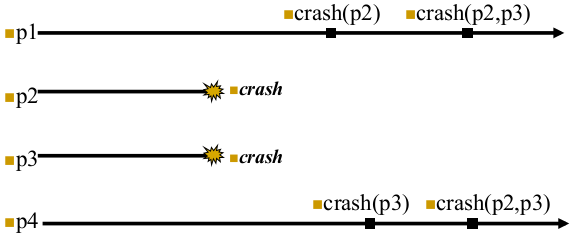
\includegraphics[width=7cm]{img/gm1.png}&
        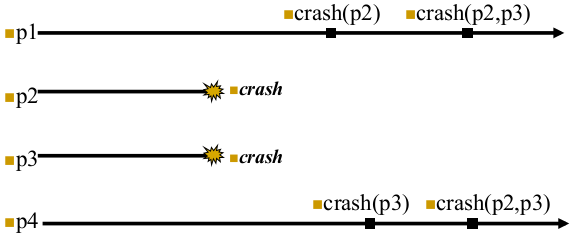
\includegraphics[width=7cm]{img/gm1.png}\\
    \end{tabular}
    \caption{Group membership}
\end{figure}
\FloatBarrier{}

\begin{itemize}
	\item Like FD, processes are informed about failures; we say that
	the processes install \textbf{views}.
	\item Like PFD, processes have accurate knowledge about failures.
	\item Unlike a PFD, the information about failures are
	coordinated, the processes install the same sequence of view.
\end{itemize}

\subsection{Properties (considering only crashes)}
\begin{description}
	\item[Local Monotonicity] If a process install view $(j,M)$ after
        installing $(k,N)$, then $j > k$ and $M \subset N$
	\item[Agreement] No two processes install views $(j,M)$ and $(j,M')$ such that
	$M \neq M'$
	\item[Completeness] If a process $p$ crashes, then there is an integer
	$j$ such that every correct process eventually installs view $(j,M)$ such that
	$p$ is not in $M$
	\item[Accuracy] If some process installs a view $(i,M)$ and $p$ is not in $M$,
	then $p$ has crashed
\end{description}

\subsection{Algorithm}
\begin{lstlisting}[caption=Group membership, mathescape]
upon event <Init> do
    view := (id:0, memb:$\Pi$)
    correct := $\Pi$
    wait := false

upon event <crash $p_i$> do
    correct := correct \ {$p_i$}

upon event (correct $\subset$ view.memb) and (wait == false) do
    wait := true
    trigger <ucPropose (view.id + 1, correct)>

upon event <ucDecided (i, m)> do
    view := (id:i, memb:m)
    wait := false
    trigger <membView view>
\end{lstlisting}

\begin{figure}[!ht]
		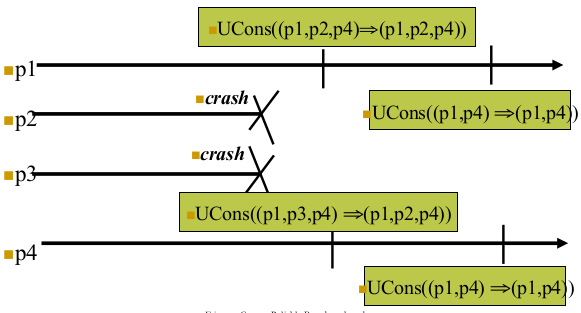
\includegraphics[width=8cm]{img/gmp_1.png}
	\caption{Group membership}
\end{figure}
\FloatBarrier{}

\subsection{Non-blocking atomic commit}
\begin{lstlisting}
Request: <nbacPropose | v>      // propose value for the commit (0 or 1)
Indication: <nbacDecide | v>    // indicate decided value
\end{lstlisting}

\begin{itemize}
    \item[NBAC1]: \textbf{Uniform agreement}: not two processes decide different values
    \item[NBAC2]: \textbf{Integrity}: no process decides two value
    \item[NBAC3]: \textbf{Abort-validity}: 0 can only be decided if some process proposes 0 or crashes
    \item[NBAC4]: \textbf{Commit-validity}: 1 can only be decided if no process proposes 0
    \item[NBAC5]: \textbf{Termination}: every correct process eventually decides
\end{itemize}
